\chapter{Introdução}
\label{chapter:intro}

A identificação de sistemas é um dos problemas mais importantes na área de controle,
sendo também relevante na de processamento de sinais. Nele, objetiva-se modelar um
processo do qual não se conhece o comportamento interno, apenas a saída e talvez a
entrada. Em alguns casos, é importante que o modelo seja robusto a sinais indesejados
presentes na saída observada --- interpretados como ruído --- para que seja possível
estimar a versão processada da entrada isolada, sem os elementos adicionais. Neste
trabalho, abordaremos algoritmos que visam a \emph{reproduzir} o processamento aplicado
a uma entrada, em posse desta e da observação da saída potencialmente ruidosa. Porém,
duas particularidades caracterizam nosso contexto: trabalharemos com gravações sonoras,
e os sistemas a serem identificados podem ser não-lineares. Essas duas condições
aumentam o nível de complexidade da solução.

Começaremos este capítulo inicial comentando a motivação por trás de abordar o problema
em questão. Em seguida, os objetivos do trabalho serão formalmente definidos. O próximo
passo será discorrer sobre a metodologia escolhida para o projeto, estabelecendo a
nomenclatura utilizada durante todo o texto, as distorções consideradas nos
experimentos, e como foram gerados os sinais de teste. Por fim, os materiais utilizados
serão mencionados, e a organização do texto será apresentada.

\section{Motivação}

Identificar o comportamento de um sistema não-linear é, por si só, um desafio
pertinente. Afinal, considere o contrário: quando pressupomos que um sistema é linear,
podemos caracterizá-lo completamente por seus polos e zeros, ou por uma equação de
diferenças. Um exemplo de algoritmo que visa a resolver o problema de forma ótima (para
o erro quadrático médio) para o caso linear é o Filtro de Wiener~\cite{hayes-1996}, o
qual discutiremos mais à frente. Modelos não-lineares, por outro lado, são muito mais
diversos: o mapeamento pode ser exponencial, trigonométrico, logarítmico... Portanto, a
modelagem é não-trivial, e requer uma abordagem mais genérica.

Duas são as soluções mais comumente propostas para resolver o problema. A primeira é o
Modelo de Hammerstein-Wiener~\cite{ogunfunmi-2007}, o qual representa o sistema por um
bloco linear seguido de um não-linear sem memória (ou vice-versa). Esse método acaba se
tornando muito limitado para nossa aplicação --- ao menos em sua forma básica ---, já
que requer que o mapeamento não-linear seja conhecido a priori. A segunda possibilidade
é a utilização da Série de Volterra~\cite{ogunfunmi-2007}, que descreve a saída do
sistema por uma equação polinomial, similar à Série de Taylor. Por ser uma série de
potências, essa abordagem facilita a generalização do sistema, porém em troca de alto
custo computacional, pois o número de coeficientes aumenta exponencialmente com a ordem
do polinômio. Portanto, seu uso deve ser feito com parcimônia. E, assim como na
primeira solução, o modelo por si só não resolve o problema, precisando ser ajustado
por meio de um algoritmo principal. Um método de identificação eficiente é capaz de
mimicar diferentes tipos de funções não-lineares, sem nenhum conhecimento sobre o
sistema.

Outro importante motivador na busca por modelos de identificação é a necessidade de
remoção de sinais espúrios em observações ruidosas. Um algoritmo robusto deve conseguir
identificar o processamento que foi aplicado ao sinal de interesse mesmo com o ruído
presente, para que então esse seja reproduzido na entrada e resulte numa estimação
limpa. Na realidade, como o principal objetivo deste trabalho é emular o processamento,
e não parametrizar o modelo, pode-se argumentar que esse seja o principal requisito do
método: robustez a ruído.

Um caso prático que envolve o problema em questão pode ser encontrado na área de
separação de fontes sonoras. Considere a mixagem presente numa produção audiovisual:
ela é composta por uma trilha sonora, uma faixa de diálogo e efeitos especiais. Em
posse da versão original da música de fundo, seria possível extrair automaticamente a
trilha sonora do áudio? É essa a pergunta que tenta ser respondida
em~\cite{lordelo-2018}. Os algoritmos apresentados foram capazes de sincronizar o sinal
original com o áudio, mas não de extrair satisfatoriamente a música. O autor suspeita
de que o principal motivo foi o processamento não-linear presente na mixagem (e
desconsiderado no método). Com isso, justifica-se a necessidade de explorar os
algoritmos no contexto de gravações sonoras.

\section{Objetivos}

O objetivo geral deste projeto é analisar comparativamente métodos de identificação de
sistemas discretos aplicados a gravações sonoras, considerando eficiência e robustez.
Neste sentido, os objetivos específicos do trabalho são: (1) apresentar modelos capazes
(ou não) de estimar não-linearidades impostas no sinal de entrada, dispondo de uma
referência; (2) elaborar métodos que permitam a aplicação desses algoritmos em sinais
digitais de áudio; e (3) comparar a qualidade das técnicas no contexto trivial de
reprodução de processamento, e também no de robustez a ruído, a fim de endereçar o
problema da remoção da trilha sonora de produções audiovisuais (com gravações
artificiais) abordado em~\cite{lordelo-2018}.

\section{Metodologia}

Antes de começarmos a discutir os algoritmos em si, é necessário apresentar a
terminologia associada aos elementos que compõem o projeto, além das restrições
impostas aos experimentos que serão executados. Estas definições são comuns a todos os
métodos analisados.

Inicialmente, é preciso contextualizar que todo o processamento se dá sobre sinais de
áudio amostrados indexados por $n$ inteiro. Quando uma gravação sonora é mixada,
dizemos que ela sofreu uma \emph{distorção}. Em nosso caso, o sinal discreto distorcido
$d[n]$\symbl{$d{[n]}$}{Versão distorcida desejada do sinal original} é o
\emph{desejado}, ou seja, o que queremos que seja estimado pelo método de
identificação. Porém, temos apenas a versão original deste sinal, identificada por
$x[n]$\symbl{$x{[n]}$}{Sinal original}, e a \emph{observação}
$y[n]$\symbl{$y{[n]}$}{Observação (possivelmente ruidosa) do sinal distorcido
	desejado}, que é possivelmente ruidosa; quando não é, $y[n] = d[n]$. A saída do
estimador é $\hat{d}[n]$\symbl{$\hat{d}{[n]}$}{Estimação da versão distorcida do sinal
	original}. Embora essa simbologia seja utilizada por todo o texto, inevitavelmente
ocorrerá sobrecarga de notação, pois priorizamos manter os símbolos originais de cada
método. De todo modo, quando os algoritmos forem adaptados ao contexto do trabalho, as
devidas associações serão feitas.

\subsection{Distorções consideradas}
\label{section:intro:distortions}

Existem diferentes tipos de processamento que podem ser aplicados a um sinal de áudio:
ganho, filtros lineares, e limitadores de amplitude são apenas alguns exemplos. Como o
objetivo do trabalho é analisar a capacidade de um método de reproduzir distorções
não-lineares (e, consequentemente, lineares), é interessante que esse seja o mais
``genérico'' possível, ou seja, que consiga imitar qualquer tipo de efeito. Para
avaliar sua generalidade, devemos fazer experimentos com gravações que possuam
diferentes distorções aplicadas de forma controlada. Seguir isto à risca e produzir uma
pletora de arquivos de teste, porém, complicaria muito os experimentos a serem feitos;
portanto, limitamo-nos a utilizar alguns dos efeitos mais comumente usados durante a
mixagem de uma gravação sonora. Estes serão apresentados a seguir.

\subsubsection{\textit{Fade-in} e \textit{fade-out} (ganho variável)}

A aplicação de um ganho é possivelmente o processamento mais trivial que um sistema
pode executar, independentemente do contexto. Em gravações sonoras, muitas vezes
encontramos este efeito na forma de \textit{fades}, que são variações graduais na
amplitude do sinal. Neste caso, em vez de se ter um ganho constante $A \geq
	0$\symbl{$A$}{Ganho constante} aplicado a toda a gravação, tem-se $A[n] \geq
	0$\symbl{$A{[n]}$}{Ganho variável}, ou seja,
\begin{equation}
	y[n] = A[n] x[n].
\end{equation}
Esta operação é linear, embora varie no tempo. Portanto, ao considerarmos este tipo de distorção em nossa análise, nosso objetivo é avaliar a capacidade de um método em reproduzir processamentos lineares variantes no tempo.

Ainda no contexto musical, temos dois tipos de \textit{fade}: o \textit{fade-in} e o
\textit{fade-out}. No primeiro, o valor inicial do ganho é o menor possível, ou seja,
$A[0] \leq A[n]\ \forall\ n \geq 0$ (considerando condições iniciais nulas para
$A[n]$), e o nível da gravação é gradualmente amplificado; assim, $A[n]$ é uma
sequência monótona crescente:
\begin{equation}
	A[n + 1] \geq A[n]\ \forall\ n \geq 0.
	\label{eq:intro-fade-in}
\end{equation}

No \textit{fade-out}, tem-se o contrário: o ganho começa em seu maior valor possível,
$A[0] \geq A[n]\ \forall\ n \geq 0$, e então o nível da gravação é gradualmente
atenuado. Neste caso, $A[n]$ torna-se uma sequência monótona decrescente:
\begin{equation}
	A[n + 1] \leq A[n]\ \forall\ n \geq 0.
	\label{eq:intro-fade-out}
\end{equation}

Ademais, além da curva que rege sua evolução, o \textit{fade-in} é normalmente definido
com as condições adicionais de que o valor inicial do ganho é $A_\text{i} =
	0$\symbl{$A_\text{i}$}{Valor inicial do ganho variável} e o final é $A_\text{f} =
	1$\symbl{$A_\text{f}$}{Valor final do ganho variável} (e vice-versa para o
\textit{fade-out}). Porém, como iremos usar \textit{fades} para colocar uma faixa ``no
plano de fundo'' em uma mixagem --- para que ela fique com um nível menor do que os das
outras fontes, mas ainda presente ---, serão usados valores iniciais e finais
diferentes de zero, como veremos nos capítulos seguintes.

\subsubsection{\textit{Soft clipping} (limitação de amplitude)}

O \textit{clipping}, ou ceifamento, é uma distorção muito associada a sinais que
passaram por amplificadores operando fora de suas respectivas faixas de operação. Este
é um problema recorrente na gravação e reprodução de sinais de áudio, onde microfones e
alto-falantes podem acabar introduzindo o efeito. Ademais, muitas vezes esta distorção
é deliberadamente aplicada por motivos artísticos --- o melhor exemplo é a
\textit{fuzzbox}, um pedal que limita a amplitude do sinal recebido --- ou para que a
mixagem cumpra as normas de \textit{loudness} do meio em que será
reproduzida~\cite{loudness-standards}.

O ceifamento nada mais é que uma limitação na amplitude: a operação delimita os valores
que podem ser alcançados pelo sinal.\footnote{Teoricamente, o valor máximo e mínimo
	podem ser diferentes; na prática, o \textit{clipping} costuma ser simétrico, de tal
	forma que os extremos são iguais em módulo.} No caso do \textit{hard clipping}, nenhuma
modificação é feita na forma de onda caso ela não ultrapasse os limiares; e quando um
destes é ultrapassado, a amostra do sinal é fixada no respectivo extremo. Já no caso do
\textit{soft clipping} o sinal sofre um mapeamento que é aproximadamente linear dentro
da faixa normal de operação, mas que suavemente limita os valores máximo e mínimo
alcançáveis. A Figura \ref{fig:intro:clipping} ilustra os dois métodos.
\begin{figure}[!ht]
	\centering
	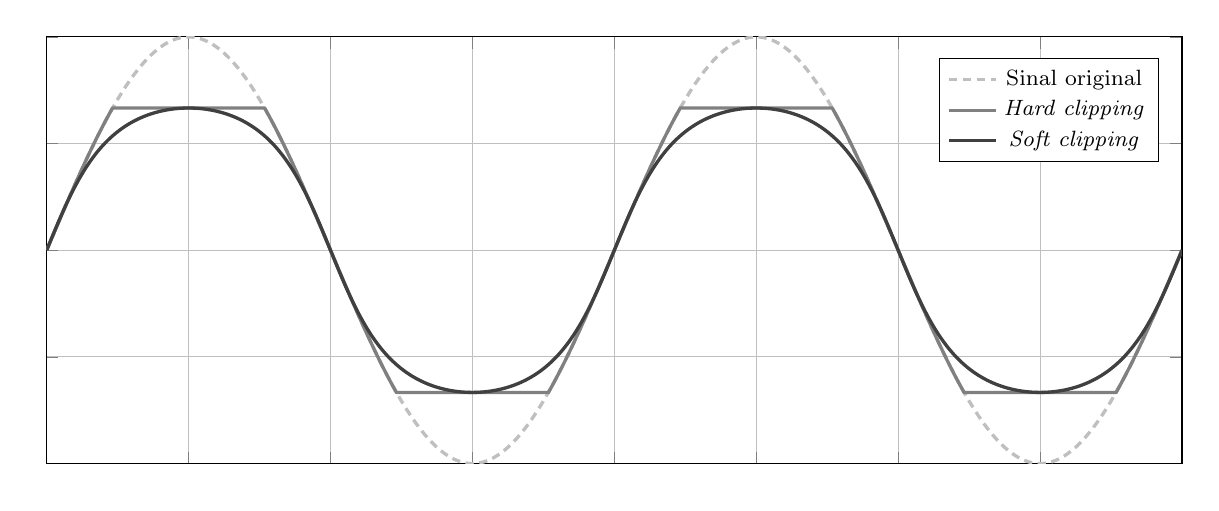
\begin{tikzpicture}[
    declare function={
        hard(\x)= (\x > 2/3) * (2/3)   +
                  and(\x <= 2/3, \x >= -2/3) * (\x) +
                  (\x < -2/3) * (-2/3);
        }
    ]

    \begin{axis}[
        ymin=-1, ymax=1, ytick={-1,-0.5,0,0.5,1},
        xmin=0, xmax=4, xtick={0,0.5,1,1.5,2,2.5,3,3.5,4},
        grid=major,
        samples=1001,
        width=16cm,
        height=7cm,
        domain=0:4,
        yticklabel=\empty,
        xticklabel=\empty,
        legend style={font=\footnotesize, at={(0.98,0.95)}, anchor=north east}
    ]
        \addplot[very thick, lightgray, densely dashed] {sin(deg(pi*x))};
        \addlegendentry{Sinal original}
        \addplot[very thick, gray] {hard(sin(deg(pi*x)))};
        \addlegendentry{\textit{Hard clipping}}
        \addplot[very thick, darkgray] {2/3 * rad(atan(tan(deg(1)) * sin(deg(pi*x))))};
        \addlegendentry{\textit{Soft clipping}}
    \end{axis}
\end{tikzpicture}

	\caption[Exemplos de \textit{hard clipping} e \textit{soft clipping}]{Exemplos de \textit{hard clipping} e \textit{soft clipping}.}
	\label{fig:intro:clipping}
\end{figure}

O \textit{soft clipping}, por aplicar uma limitação menos ``brusca'', afeta menos a
qualidade do sinal, e, por isso, é mais frequentemente usado quando a distorção é
propositalmente aplicada. Portanto, este será o efeito considerado nos experimentos.

\subsubsection{Codificação com perdas}

Métodos de codificação são utilizados para reduzir a quantidade de bits que compõem um
arquivo, e consequentemente comprimi-lo (não confundir com compressão da magnitude do
áudio). Deste modo, necessita-se de menos espaço físico para armazenar o dado e menos
banda para transmiti-lo.

Na codificação sem perdas, nenhuma informação é descartada, apenas redundâncias são
reduzidas; assim, o dado pode ser decodificado e reconstruído perfeitamente. Já na
codificação com perdas, são utilizadas particularidades da percepção humana para
remover partes imperceptíveis (para a maioria das pessoas) do sinal, fazendo com que o
dado codificado \emph{pareça} igual a sua versão original, embora esteja incompleto. No
caso de gravações sonoras, os algoritmos de codificação consideram propriedades
psicoacústicas durante o processo, e com isso conseguem alcançar taxas de compressão
cerca de três vezes maiores do que no caso sem perdas~\cite{bosi-2002}.

Ambas as formas de codificação são muito utilizadas; a sem perdas, porém, não modifica
o sinal em sua versão decodificada, e, portanto, não pode ser considerada um tipo de
distorção. Já o método com perdas altera o sinal de forma extremamente complexa e
não-linear: curvas de mascaramento e alocação de bits~\cite{bosi-2002} são apenas dois
dos diversas recursos utilizados no MP3\abbrev{MP3}{MPEG-2 \textit{Audio Layer} III},
por exemplo. Dada sua relevância, sinais codificados em MP3 serão utilizados nos
testes.

\subsection{Método de geração dos sinais de teste}
\label{section:intro:gensignals}

Como explicitado na seção anterior, gravações artificiais foram geradas de forma
controlada para a execução dos experimentos do projeto. Discorreremos agora brevemente
sobre o método de geração destes sinais. A observação $y[n]$ é formada a partir de uma
mixagem entre o sinal original $x[n]$ e possivelmente um sinal descorrelacionado
$r[n]$\symbl{$r{[n]}$}{Ruído introduzido durante o processo de mixagem}, interpretado
como ruído. Podemos representar todo o processo de mixagem com uma função genérica:
\begin{equation}
	y[n] = f(x, r)\symbl{$f(x, r)$}{Função que engloba todo o processo de mixagem aplicado ao sinal original e o ruído}.
\end{equation}
Este mapeamento pode ser desde uma simples soma entre os sinais até uma operação mais complexa, contanto que se limite às distorções explicitadas.

Em posse de $x[n]$ e $y[n]$, o objetivo do estimador é gerar a gravação distorcida
desejada $d[n]$ resultante de $f(x, 0)$, ou seja, o mapeamento quando o ruído é
inexistente. A Figura~\ref{fig:intro:experiments-model} ilustra a dinâmica dos
experimentos: com o sinal original e o ruído, fabrica-se a mixagem; e, com apenas o
sinal original, produz-se também a versão distorcida desejada (que, no geral, não
possuímos, mas precisamos gerar para que possamos avaliar os métodos). Então, os sinais
$x[n]$ e $y[n]$ são passados para o modelo, simbolizado pelo bloco ``Estimador'', que
tenta reproduzir $d[n]$, gerando $\hat{d}[n]$. A eficiência do método é avaliada
comparando-se medidas entre $(d, \hat{d})$ e $(d, x)$.

\medskip
\begin{figure}[!ht]
	\centering
	\begin{tikzpicture}[node distance=1.25cm and 1.25cm]
    \node[dspnodeopen, dsp/label=left] (x) {$x[n]$};
    \node[dspnodefull, right=of x] (x-split) {};

    \node[dspfilter, right=of x-split] (w) {Estimador};
    \node[dspfilter, above=of w] (f) {$f(x, r)$};
    \node[dspfilter, below=of w, dashed] (f-zero) {$f(x, 0)$};

    \node[dspnodeopen, dsp/label=left, above=of f, yshift=-0.5cm] (r) {$r[n]$};

    \draw[dspline] (x) -- (x-split);
    \draw[dspconn] (x-split) -- (w);
    \draw[dspconn] (x-split) |- (f-zero);
    \draw[dspconn] (x-split) |- (f);
    \draw[dspconn] (r) -- (f);

    \draw[dspconn] (f) -- node[midway,right] {$y[n]$} (w);

    \node[dspnodeopen, dsp/label=right, right=of f-zero] (d) {$d[n]$};
    \node[dspnodeopen, dsp/label=right, right=of w] (dhat) {$\hat{d}[n]$};

    \draw[dspconn] (w) -- (dhat);
    \draw[dspconn] (f-zero) -- (d);
\end{tikzpicture}

	\caption[Diagrama de blocos do sistema dos experimentos]{Diagrama de blocos do sistema modelado para os experimentos com os filtros utilizados no projeto.}
	\label{fig:intro:experiments-model}
\end{figure}

\section{Material utilizado}

Todos os algoritmos discutidos foram implementados em MATLAB pelo autor, exceto quando
indicado. O repositório com todos os códigos (autorais) do trabalho encontra-se
em~\cite{nonlinear-filters-repo}; além disso, os resultados dos experimentos (as
gravações estimadas) podem ser consultadas em~\cite{nonlinear-results}. Os experimentos
foram executados nas máquinas do Laboratório de Sinais, Multimídia e Telecomunicações
(SMT\abbrev{SMT}{Sinais, Multimídia e Telecomunicações}) da Universidade Federal do Rio
de Janeiro, na versão R2017a do MATLAB. O processamento das gravações foi executado com
os programas Audacity~\cite{audacity} e GoldWave~\cite{goldwave}. Este documento foi
produzido em \LaTeX.

\section{Organização do texto}

Neste primeiro capítulo, o problema foi formulado, e as nomenclaturas e restrições
pertinentes a todo o texto foram definidas. No Capítulo~\ref{chapter:metrics},
discutiremos as medidas usadas para avaliar o desempenho dos métodos. Em seguida, no
Capítulo~\ref{chapter:wiener}, será desenvolvido o Filtro de Wiener, um filtro ótimo,
porém linear. Então, partiremos para nosso primeiro modelo não-linear, com o Filtro de
Correntropia, no Capítulo~\ref{chapter:correntropyfilter}. E no
Capítulo~\ref{chapter:unscented}, veremos o Filtro de Kalman \textit{Unscented}, o
último método a ser avaliado. Finalmente, as conclusões serão apresentadas no
Capítulo~\ref{chapter:conclusion}.
